%!TEX program = xelatex
\documentclass[a4paper,12pt]{report}
\usepackage{ctex}
%\usepackage{xeCJK}
\usepackage{times}
\usepackage{graphicx,float}
\usepackage{setspace}
\usepackage{fancyhdr}
% \usepackage{graphicx}
\usepackage{wrapfig}
\usepackage{array}
\usepackage{fontspec,xunicode,xltxtra}
\usepackage{titlesec}
\usepackage{titletoc}
\usepackage[titletoc]{appendix}
\usepackage[top=30mm,bottom=30mm,left=20mm,right=20mm]{geometry}
\usepackage{cite}
\usepackage{listings}
\usepackage{xcolor}
\usepackage{amsmath}
\lstset{
    basicstyle=\small\ttfamily, % 基本样式
    frame=single, % 代码块边框
    tabsize=4, % 制表符宽度
    numbers=left, % 行号位置
    language=Java, % 代码语言
    showstringspaces=false, % 不显示字符串中的空格
    commentstyle=\color{gray}, % 注释颜色
    keywordstyle=\color{blue}, % 关键字颜色
    stringstyle=\color{red}, % 字符串颜色
}
\usepackage[framed,numbered,autolinebreaks,useliterate]{mcode} % 插入代码
\XeTeXlinebreaklocale "zh"
\XeTeXlinebreakskip = 0pt plus 1pt minus 0.1pt

%---------------------------------------------------------------------
%	页眉页脚设置
%---------------------------------------------------------------------
\fancypagestyle{plain}{
	\pagestyle{fancy}      %改变章节首页页眉
}

\pagestyle{fancy}
\lhead{\kaishu~``计算机图形与图像技术''课程报告~}
\rhead{\kaishu~~梁涵杰、刘维江~~}
\cfoot{\thepage}

%---------------------------------------------------------------------
%	章节标题设置
%---------------------------------------------------------------------
%\titleformat{\section}{\centering\zihao{-1}\heiti}{报告\chinese{section}}{1em}{}
%\titlespacing{\section}{0pt}{*0}{*6}

%---------------------------------------------------------------------
%	摘要标题设置
%---------------------------------------------------------------------
\renewcommand{\contentsname}{\centerline{\zihao{2} 目\quad 录}}

%---------------------------------------------------------------------
%	参考文献设置
%---------------------------------------------------------------------
\renewcommand{\bibname}{\centerline{\zihao{2}{参\hspace{0.5em}考\hspace{0.5em}文\hspace{0.5em}献}}}

%---------------------------------------------------------------------
%	引用文献设置为上标
%---------------------------------------------------------------------
\makeatletter
\def\@cite#1#2{\textsuperscript{[{#1\if@tempswa , #2\fi}]}}
\makeatother

%---------------------------------------------------------------------
%	目录页设置
%---------------------------------------------------------------------
%\titlecontents{chapter}[0em]{\songti\zihao{-4}}{\thecontentslabel\ }{}
%{\hspace{.5em}\titlerule*[4pt]{$\cdot$}\contentspage}
%\titlecontents{section}[2em]{\vspace{0.1\baselineskip}\songti\zihao{-4}}{\thecontentslabel\ }{}
%{\hspace{.5em}\titlerule*[4pt]{$\cdot$}\contentspage}
%\titlecontents{subsection}[4em]{\vspace{0.1\baselineskip}\songti\zihao{-4}}{\thecontentslabel\ }{}
%{\hspace{.5em}\titlerule*[4pt]{$\cdot$}\contentspage}
\renewcommand\thesection{\arabic{section}}
\renewcommand\thesubsection{\arabic{section}.\arabic{subsection}}

\begin{document}


%---------------------------------------------------------------------
%	封面设置
%---------------------------------------------------------------------
\begin{titlepage}
	\begin{center}
		
    
\includegraphics[width=1.0\textwidth]{figure//nankai.jpg}\\
    % \vspace{10mm}
    % \textbf{\zihao{2}\kaishu{软件学院}}\\[0.8cm]
    \vspace{50mm}
    \textbf{\zihao{1}\heiti{ 《计算机图形与图像技术》课程报告}}\\[3cm]
    \textbf{\zihao{2}\heiti{ 基于双边滤波器的图像卡通化工具}}\\[3cm]
	\vspace{\fill}
	
\setlength{\extrarowheight}{3mm}
{\songti\zihao{3}	
\begin{tabular}{rl}
	
	
	{\makebox[4\ccwd][s]{组员 1:}}& ~\kaishu 梁涵杰 2120230780~~ \\

    {\makebox[4\ccwd][s]{组员 2:}}& ~\kaishu 刘维江 2120230782~~ \\


\end{tabular}
 }\\[2cm]
\vspace{\fill}
\zihao{4}
2023\textasciitilde 2024第二学期\\
	\end{center}	
\end{titlepage}


%---------------------------------------------------------------------
%  目录页
%---------------------------------------------------------------------
\tableofcontents % 生成目录

%---------------------------------------------------------------------
%
%---------------------------------------------------------------------
\newpage

\section{引言}
图像卡通化是一种将真实图像转换为卡通风格图像的技术,广泛应用于图像处理、摄影后期、视觉艺术等领域。传统的图像平滑方法通常会模糊图像的边缘,导致图像细节丢失。双边滤波器通过结合空间域和像素值域的加权,可以在去除噪声的同时保留边缘细节,因此非常适合用于图像卡通化处理。
\section{双边滤波器原理}
双边滤波器(Bilateral Filter)是一种在图像处理中的非线性滤波器,它可以在平滑图像的同时保留边缘。与传统的高斯滤波不同,双边滤波器不仅考虑像素之间的空间距离,还考虑像素值的相似度。这样可以避免模糊图像中的边缘,使图像看起来更加清晰自然。
\subsection{基本概念}
双边滤波器的输出像素值是输入图像中像素值的加权平均,权重由空间距离和像素值差异共同决定。权重的计算依赖于两个高斯函数:一个基于空间距离,另一个基于像素值差异。

\subsection{公式及含义}

\begin{equation}
    I_{\text{filtered}}(x) = \frac{1}{W_p} \sum_{x_i \in \mathcal{N}(x)} I(x_i) \cdot f_r(|I(x_i) - I(x)|) \cdot f_s(|x_i - x|)
\end{equation}
其中,$I_{\text{filtered}}(x)$ 是滤波后的像素值。
$I(x)$ 是原始图像的像素值。
$\mathcal{N}(x)$ 是像素 $x$ 的邻域。
$f_r$ 是基于像素值差异的高斯函数。
$f_s$ 是基于空间距离的高斯函数。
$W_p$ 是归一化因子,确保权重之和为1。

\subsection{高斯权重函数}
\begin{itemize}
    \item 空间权重依赖于像素之间的空间距离,使用空间域的高斯函数 $f_s$。
        \begin{equation}
        f_s(|x_i - x|) = \exp\left(-\frac{|x_i - x|^2}{2 \sigma_s^2}\right) 
        \end{equation}
    \item 像素值权重依赖于像素值之间的差异,使用像素值域的高斯函数 $f_r$。
        \begin{equation}
        f_r(|I(x_i) - I(x)|) = \exp\left(-\frac{|I(x_i) - I(x)|^2}{2 \sigma_r^2}\right) 
        \end{equation}
\end{itemize}

\subsection{双边滤波的步骤}
\begin{enumerate}
    \item 定义滤波窗口:选择一个直径为 ( d ) 的滤波窗口(邻域大小)。
    \item 计算权重:对于窗口中的每个像素,计算其与中心像素的空间权重和像素值权重。
    \item 加权平均:根据权重计算加权平均值,得到滤波后的像素值。
    \item 归一化:将所有权重归一化,确保权重之和为1。
\end{enumerate}

\section{实现思路以及代码实现}
\subsection{读取图像}
首先读取需要进行卡通画的原始图像,这里我们选择 使用 OpenCV 中的库函数 cv2.imread 来加载图像并返回一个包含该图像数据的 NumPy 数组,方便后续的处理。

然后对加载的图像进行预处理,将读取的图像数据从整数类型转换为浮点数类型,并将像素值归一化到 [0, 1] 的范围。
\begin{lstlisting}[language=Python]
input_image = cv2.imread('test.png')
if input_image is None:
    raise ValueError("无法打开或找到图像。")

input_image = input_image.astype(np.float32) / 255.0 
\end{lstlisting}

\subsection{平滑处理}
使用双边滤波器通过结合空间距离和像素值差异进行加权平均,来实现图像的平滑处理。

\begin{lstlisting}[language=Python]
def apply_bilateral_filter(image, diameter, sigma_i, sigma_s):
    rows, cols = image.shape[:2]
    half_diameter = diameter // 2
    filtered_image = np.zeros_like(image, dtype=np.float32)

    # 预计算空间权重
    gauss_spatial = np.zeros((diameter, diameter), dtype=np.float32)
    for i in range(diameter):
        for j in range(diameter):
            x = i - half_diameter
            y = j - half_diameter
            gauss_spatial[i, j] = np.exp(-(x**2 + y**2) / (2 * sigma_s**2))

    # 对每个像素进行双边滤波
    for ch in range(3):  # 对每个通道
        for i in range(rows):
            for j in range(cols):
                Wp = 0
                filtered_pixel = 0

                for k in range(-half_diameter, half_diameter + 1):
                    for l in range(-half_diameter, half_diameter + 1):
                        ni = i + k
                        nj = j + l

                        if 0 <= ni < rows and 0 <= nj < cols:
                            intensity_diff = image[ni, nj, ch] - image[i, j, ch]
                            gauss_range = np.exp(-(intensity_diff**2) / (2 * sigma_i**2))
                            weight = gauss_spatial[k + half_diameter, l + half_diameter] * gauss_range
                            Wp += weight
                            filtered_pixel += weight * image[ni, nj, ch]

                filtered_image[i, j, ch] = filtered_pixel / Wp

    return filtered_image
\end{lstlisting}

\subsection{边缘检测}
将输入的彩色图像转换为灰度图像,使用中值滤波器对其进行平滑处理,然后通过自适应阈值方法检测图像的边缘。
\begin{lstlisting}[language=Python]
def detect_edges(image):
    gray = cv2.cvtColor(image, cv2.COLOR_BGR2GRAY)
    gray_uint8 = (gray * 255).astype(np.uint8)
    gray_blurred = cv2.medianBlur(gray_uint8, 7)
    edges = cv2.adaptiveThreshold(
        gray_blurred, 255,
        cv2.ADAPTIVE_THRESH_MEAN_C,
        cv2.THRESH_BINARY,
        blockSize=9,
        C=2
    )
    return edges
\end{lstlisting}

\subsection{合并结果}
最后将平滑后的图像与边缘图像合并,生成卡通化效果。
\begin{lstlisting}[language=Python]
def combine_edges_and_smooth(image, edges):
    edges_colored = cv2.cvtColor(edges, cv2.COLOR_GRAY2BGR)
    edges_colored = edges_colored / 255.0  # 归一化到 [0, 1]
    combined_image = np.clip(image * edges_colored, 0, 1)
    return combined_image
\end{lstlisting}

\subsection{输出图像}
\begin{lstlisting}[language=Python]
def cartoonize_image(image, diameter=9, sigma_i=75, sigma_s=75):
    # 应用双边滤波
    smoothed_image = apply_bilateral_filter(image, diameter, sigma_i, sigma_s)
    
    # 检测边缘
    edges = detect_edges(image)
    
    # 合并平滑图像和边缘图像
    cartoon_image = combine_edges_and_smooth(smoothed_image, edges)
    
    return cartoon_image
\end{lstlisting}


\section{实验结果}
\begin{figure}[H]
    \centering
    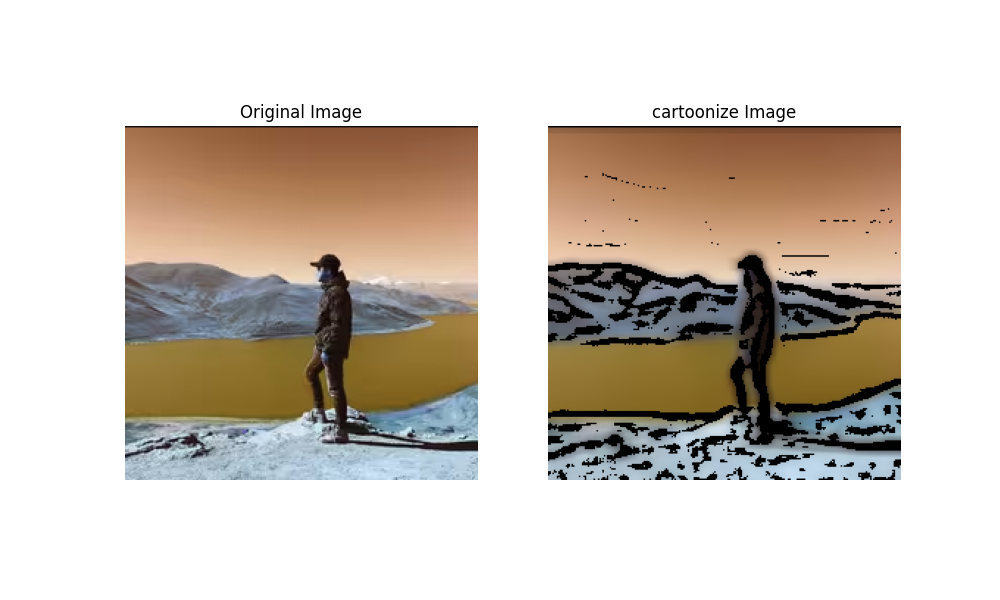
\includegraphics[width=0.8\textwidth]{figure/res_1.png}
    \caption{实验 3}
    \label{fig:login}
\end{figure}

\begin{figure}[H]
    \centering
    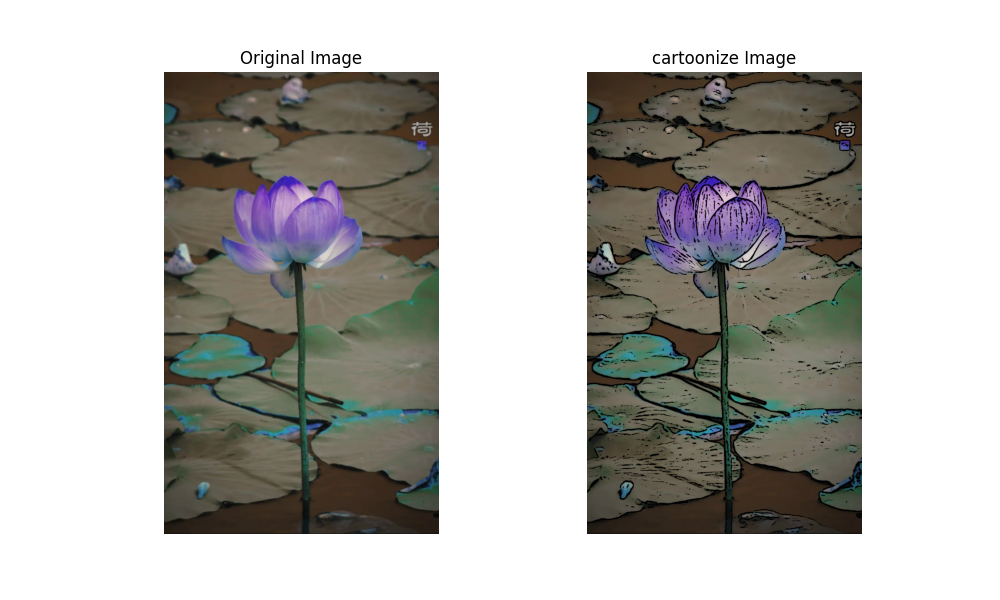
\includegraphics[width=0.8\textwidth]{figure/res_2.png}
    \caption{实验 2}
    \label{fig:login}
\end{figure}

\begin{figure}[H]
    \centering
    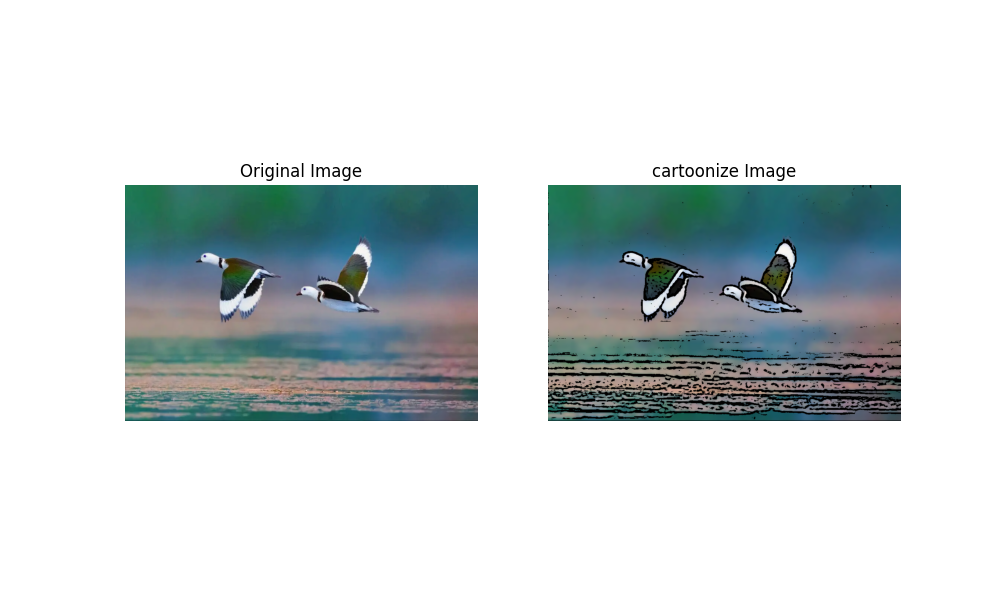
\includegraphics[width=0.8\textwidth]{figure/res_3.png}
    \caption{实验 3}
    \label{fig:login}
\end{figure}


\section{总结}
通过本次课程实验,我们进一步学习理解了双边滤波器的原理和应用场景,深入掌握了如何手动实现双边滤波器,并将其应用于图像卡通化处理。双边滤波器是一种能够同时考虑空间距离和像素强度差异的非线性滤波技术,与传统的线性滤波器相比,它在去噪的同时能够更好地保留图像的边缘细节。

在实验过程中,我们通过手动实现双边滤波器,进一步理解了其核心原理,包括空间权重和强度权重的计算方法。空间权重基于高斯函数,考虑像素间的几何距离;强度权重则基于像素值的差异,确保边缘部分的像素在滤波过程中不会被模糊掉。通过调整滤波窗口的直径及高斯函数的标准差参数,我们可以灵活地控制平滑效果和边缘保留效果。

此外,我们将双边滤波器与自适应阈值边缘检测结合,开发出一个简单的图像卡通化工具。具体步骤包括:首先对图像应用双边滤波,平滑图像的同时保留边缘;然后使用自适应阈值方法检测图像的边缘,生成二值化的边缘图像;最后将平滑后的图像与边缘图像结合,生成卡通化效果。通过这种方法,原始图像中的噪声被有效去除,同时关键的边缘和轮廓得到了突显,使得图像呈现出类似手绘的卡通效果。

本次实验不仅让我们掌握了双边滤波器的实现和应用,还拓展了我们对图像处理技术的理解,通过实验的实践操作,我们加深了对理论知识的理解,并积累了宝贵的编程经验和技术技巧。

		

\end{document}
